\chapter[Mie Coefficients][Mie Coefficients]{Mie Coefficients}\label{ap:MieCoefficients}
%
The Mie coefficients describe electromagnetic scattering by a sphere and are often used for computing quantities such as the absorption, extinction, and scattering cross sections.\cite{Mie1908, Kattawar1970, Mackowski1994, Bohren2004, Wriedt2012}  The Mie coefficients are known by many names (scattering coefficients, field coefficients, reflection coefficients, Lorentz-Mie coefficients) and many symbols ($a_{n}$ and $b_{n}$, $\alpha_{n}$ and $\beta_{n}$, $v_{n}$ and $u_{n}$, or $R_{n}^{(M)}$ and $R_{n}^{(N)}$) across the literature. In this work, we will refer to the effective Mie coefficients for layered spheres as $\widetilde{R}_{n}^{(M)}$ and $\widetilde{R}_{n}^{(N)}$ and the Mie coefficients for homogeneous spheres as $R_{n}^{(M)}$ and $R_{n}^{(N)}$.

In this appendix, we will consider a layered sphere with $N_{l}$ layers ($N_{l} \ge 0$). See Fig. \ref{fig:Sphere_Geometry}. Any layer $i$ has outer radius $x_{i}$. The outer radius of the outermost layer is also referred to as $\rho$, to remain consistent with in the chapters of this document. A homogeneous sphere is simply the special case of $N_{l}=0$.

\begin{figure}
\centering
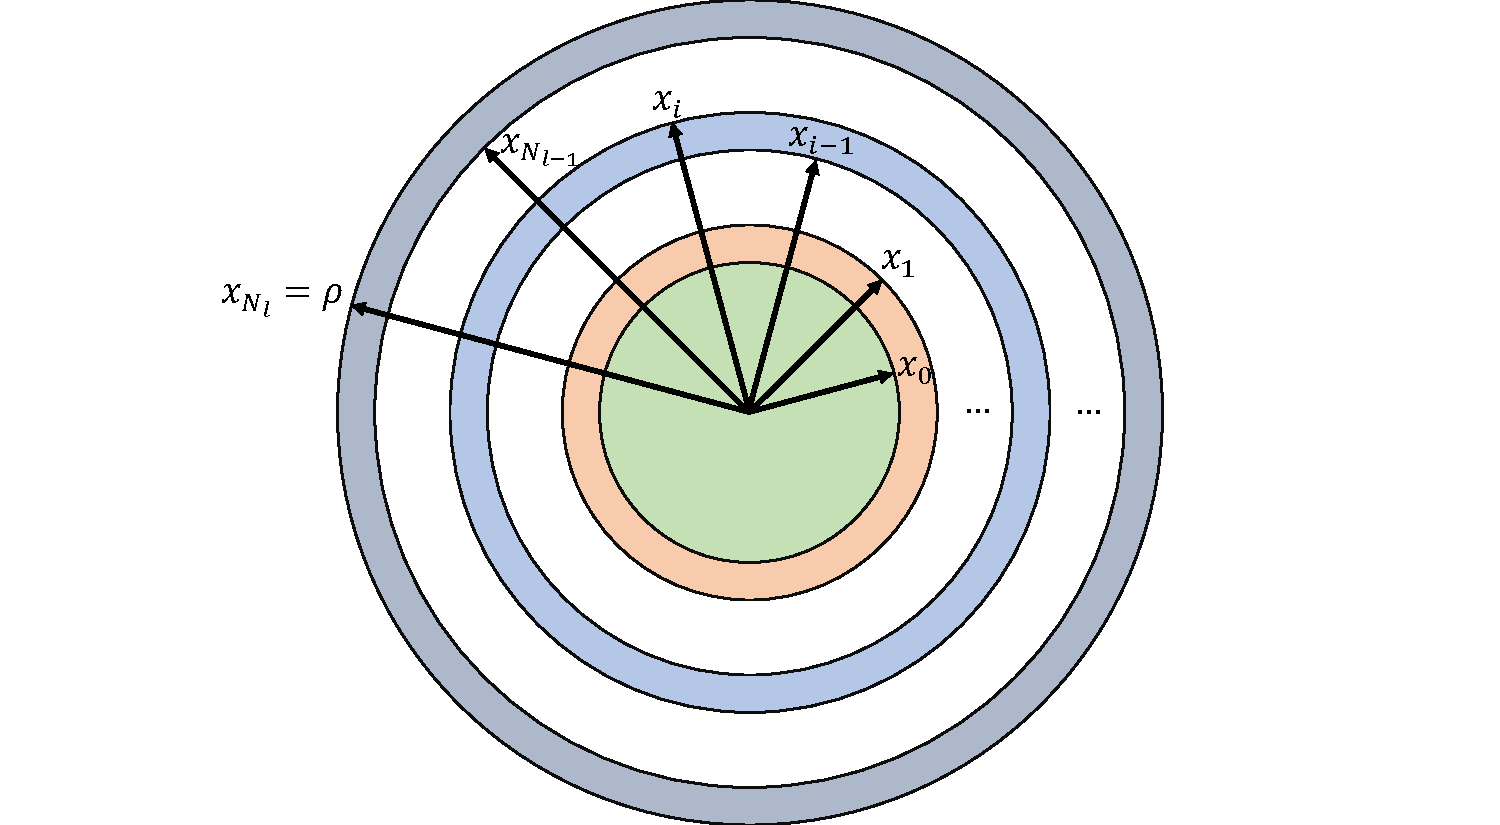
\includegraphics[width=0.8\textwidth]{./Figures/Sphere_Geometry.pdf}
\caption{\label{fig:Sphere_Geometry}Configuration of a layered sphere. The layered sphere is composed of a core and $N_{l}$ spherically symmetric layers. Each component of the sphere has an outer radius $x_{i}$ where $i=0$ for the core or $i$ takes the label of the layer, counting outward from the core. The radius of the outermost layer is also denoted $\rho$, to match the notation in the rest of this document.}
\end{figure}

%
The expressions for the effective Mie coefficients of uncoated and single-coating spheres are well known from the literature.\cite{Mie1976, Kaiser1993, Bohren2004, Zhou2006, Zheng2015} The full, multilayered Mie coefficients can be determined recursively in a manner similar to that of Fresnel reflection coefficients for planar stratified media.\cite{Narayanaswamy2013b} The recurrence relation is given by
%
\begin{subequations} \label{eq:MultilayeredMie}
\begin{align}
\widetilde{R}_{n}^{(M)}(x_{i}) &= \frac{ R_{n}^{(M)}(x_{i}) + \widetilde{R}_{n}^{(M)}(x_{i-1}) \alpha_{n}^{(M)}(x_{i}) }{ 1 + \widetilde{R}_{n}^{(M)}(x_{i-1}) \beta_{n}^{(M)}(x_{i}) }
\\
\widetilde{R}_{n}^{(N)}(x_{i}) &= \frac{ R_{n}^{(N)}(x_{i}) + \widetilde{R}_{n}^{(N)}(x_{i-1}) \alpha_{n}^{(N)}(x_{i}) }{ 1 + \widetilde{R}_{n}^{(N)}(x_{i-1}) \beta_{n}^{(N)}(x_{i}) }
\end{align}
\end{subequations}
%
where
%
\begin{subequations}\label{eq:Mie_definition1}
\begin{align}
R_{n}^{(M)}(x_{i})
&= - \frac{z_{n}^{(1)}(k_{i+1} x_{i})}{z_{n}^{(3)}(k_{i+1} x_{i})}
\left[ \frac{ \frac{1}{Z_{i+1}} \frac{\zeta_{n}^{(1)}(k_{i+1} x_{i})}{z_{n}^{(1)}(k_{i+1} x_{i})} - \frac{1}{Z_{i}} \frac{\zeta_{n}^{(1)}(k_{i} x_{i})}{z_{n}^{(1)}(k_{i} x_{i})} }{ \frac{1}{Z_{i+1}} \frac{\zeta_{n}^{(3)}(k_{i+1} x_{i})}{z_{n}^{(3)}(k_{i+1} x_{i})} - \frac{1}{Z_{i}} \frac{\zeta_{n}^{(1)}(k_{i} x_{i})}{z_{n}^{(1)}(k_{i} x_{i})} } \right]
\\
R_{n}^{(N)}(x_{i})
&= - \frac{\zeta_{n}^{(1)}(k_{i+1} x_{i})}{\zeta_{n}^{(3)}(k_{i+1} x_{i})}
\left[ \frac{ \frac{1}{Z_{i+1}} \frac{z_{n}^{(1)}(k_{i+1} x_{i})}{\zeta_{n}^{(1)}(k_{i+1} x_{i})} - \frac{1}{Z_{i}} \frac{z_{n}^{(1)}(k_{i} x_{i})}{\zeta_{n}^{(1)}(k_{i} x_{i})} }{ \frac{1}{Z_{i+1}} \frac{z_{n}^{(3)}(k_{i+1} x_{i})}{\zeta_{n}^{(3)}(k_{i+1} x_{i})} - \frac{1}{Z_{i}} \frac{z_{n}^{(1)}(k_{i} x_{i})}{\zeta_{n}^{(1)}(k_{i} x_{i})} } \right]
\end{align}
\end{subequations}
%
\begin{subequations}
\begin{align}
\alpha_{n}^{(M)}(x_{i})
&= - \frac{z_{n}^{(1)}(k_{i+1} x_{i})}{z_{n}^{(3)}(k_{i+1} x_{i})} \frac{z_{n}^{(3)}(k_{i} x_{i})}{z_{n}^{(1)}(k_{i} x_{i})}
\left[ \frac{ \frac{1}{Z_{i+1}} \frac{\zeta_{n}^{(1)}(k_{i+1} x_{i})}{z_{n}^{(1)}(k_{i+1} x_{i})} - \frac{1}{Z_{i}} \frac{\zeta_{n}^{(3)}(k_{i} x_{i})}{z_{n}^{(3)}(k_{i} x_{i})} }{ \frac{1}{Z_{i+1}} \frac{\zeta_{n}^{(3)}(k_{i+1} x_{i})}{z_{n}^{(3)}(k_{i+1} x_{i})} - \frac{1}{Z_{i}} \frac{\zeta_{n}^{(1)}(k_{i} x_{i})}{z_{n}^{(1)}(k_{i} x_{i})} } \right]
\\
\alpha_{n}^{(N)}( x_{i})
&= - \frac{\zeta_{n}^{(1)}(k_{i+1} x_{i})}{\zeta_{n}^{(3)}(k_{i+1} x_{i})} \frac{\zeta_{n}^{(3)}(k_{i} x_{i})}{\zeta_{n}^{(1)}(k_{i} x_{i})}
\left[ \frac{ \frac{1}{Z_{i+1}} \frac{z_{n}^{(1)}(k_{i+1} x_{i})}{\zeta_{n}^{(1)}(k_{i+1} x_{i})} - \frac{1}{Z_{i}} \frac{z_{n}^{(3)}(k_{i} x_{i})}{\zeta_{n}^{(3)}(k_{i} x_{i})} }{ \frac{1}{Z_{i+1}} \frac{z_{n}^{(3)}(k_{i+1} x_{i})}{\zeta_{n}^{(3)}(k_{i+1} x_{i})} - \frac{1}{Z_{i}} \frac{z_{n}^{(1)}(k_{i} x_{i})}{\zeta_{n}^{(1)}(k_{i} x_{i})} } \right]
\end{align}
\end{subequations}
%
\begin{subequations}\label{eq:Mie_definition3}
\begin{align}
\beta_{n}^{(M)}( x_{i})
&= \frac{z_{n}^{(3)}(k_{i} x_{i})}{z_{n}^{(1)}(k_{i} x_{i})}
\left[ \frac{ \frac{1}{Z_{i+1}} \frac{\zeta_{n}^{(3)}(k_{i+1} x_{i})}{z_{n}^{(3)}(k_{i+1} x_{i})} - \frac{1}{Z_{i}} \frac{\zeta_{n}^{(3)}(k_{i} x_{i})}{z_{n}^{(3)}(k_{i} x_{i})} }{ \frac{1}{Z_{i+1}} \frac{\zeta_{n}^{(3)}(k_{i+1} x_{i})}{z_{n}^{(3)}(k_{i+1} x_{i})} - \frac{1}{Z_{i}} \frac{\zeta_{n}^{(1)}(k_{i} x_{i})}{z_{n}^{(1)}(k_{i} x_{i})} } \right]
\\
\beta_{n}^{(N)}( x_{i})
&= \frac{\zeta_{n}^{(3)}(k_{i} x_{i})}{\zeta_{n}^{(1)}(k_{i} x_{i})}
\left[ \frac{ \frac{1}{Z_{i+1}} \frac{z_{n}^{(3)}(k_{i+1} x_{i})}{\zeta_{n}^{(3)}(k_{i+1} x_{i})} - \frac{1}{Z_{i}} \frac{z_{n}^{(3)}(k_{i} x_{i})}{\zeta_{n}^{(3)}(k_{i} x_{i})} }{ \frac{1}{Z_{i+1}} \frac{z_{n}^{(3)}(k_{i+1} x_{i})}{\zeta_{n}^{(3)}(k_{i+1} x_{i})} - \frac{1}{Z_{i}} \frac{z_{n}^{(1)}(k_{i} x_{i})}{\zeta_{n}^{(1)}(k_{i} x_{i})} } \right]
\end{align}
\end{subequations}

In Eqs. (\ref{eq:Mie_definition1})-(\ref{eq:Mie_definition3}), $Z=Z_0 \sqrt{\mu/\varepsilon}$ is the electromagnetic impedance for a dielectric material and $Z_0=\sqrt{\mu_0/\varepsilon_0}$ is the impedance of free space. $k_{i}$ refers to the value of $k$ within the core ($i=0$), layer $i$ ($1<i\le N_{l}$), or in the free-space region $f$ ($i=N_{l}+1$). The recursion relation is terminated by $\widetilde{R}_{n}^{(M)}(x_{0}) = R_{n}^{(M)}(x_{0})$ and $\widetilde{R}_{n}^{(N)}(x_{0}) = R_{n}^{(N)}(x_{0})$. The the case of a homogeneous sphere can be recovered from the recursion relations if the core and layers all have the same optical properties. In that case, Eq. \ref{eq:MultilayeredMie} simply to
%
\begin{subequations}
\begin{align}
\widetilde{R}_{n}^{(M)}(\rho) &= R_{n}^{(M)}(\rho)
\\
\widetilde{R}_{n}^{(N)}(\rho) &= R_{n}^{(N)}(\rho)
\end{align}
\end{subequations}